%-------------------------------------------------------------------------------
%	CAPITOLO 42
%-------------------------------------------------------------------------------

\chapter{Il Capitano}
Anche questo capitolo è presente nell'indice ma purtroppo non è mai stato scritto. Tuttavia, nel raccoglitore di mio nonno ho trovato una lettera insieme ai manoscritti.\\
\indent Questa lettera è indirizzata a Stefano Mingazzi ed è firmata \emph{G. De Maria}. Giuseppe De Maria (cav.)\index[Personaggi]{De Maria Giuseppe} fu sindaco di Alfonsine nel 1902 e fu farmacista.\\
\indent Probabilmente Mingazzi chiese a Giuseppe De Maria qualche informazione sul \emph{Capitano Lucidi}, ovvero \index[Personaggi]{Lucidi Pietro (assessore)}Pietro Lucidi, che fu assessore delegato.\\

\indent Riporto fedelmente il contenuto della lettera:\\\\
\textit{
\rightline{Roma 28.10.1942}
Gentilissimo Stefano,\\
Subito dopo il ritorno di Nando e della Clara a Roma sono stato colto dell'influenza. Questa è la sola ragione per cui la mia risposta le giunge con tanto ritardo.\\
Io sarei stato ben lieto di poterle fornire notizie inedite sul Capitano Lucidi; ma da quello che m'ha raccontato la Clara, Lei, benché comparso sulla scena del mondo ben tardi, conosce di questa macchietta tutta la ridicola istoria.\\
In una zirudela stampata alla macchina verso il 1880 e attribuita al maestro \index[Personaggi]{Castellani Giulio (avvocato)}Castellani ecco com'era dipinto quest'imbecille:
\begin{verse}
	E Badoia e vó sté d'sora\\
	E e dis: "ostia, va in malora!"\\
	Lò beet cun e su amor\\
	a squicer a totti agli or\\
	Il sa tott che é su zarvell\\
	Uiè scap d'sotta e cappell
\end{verse}
Rovistando nel mio disordinato archivio ho trovato un brutto sonetto che riguarda il Capitano, che io composi, se non erro nel 1887. Esso mi fu ispirato da una scena violenta avvenuta sulla piazza di Alfonsine, provocata da rivalità in amor, fra il \index[Personaggi]{Capitano}Capitano e certo Cavour, calzolaio, conosciuto anche come figlio di \index[Personaggi]{Bigano (fabbro)}Bigano, il quale, Cavour, mi pare che morisse al manicomio.\\
Nel sonetto è il Capitano che parla:
\begin{verse}
	Con la zanetta di legnoso albano(1),\\
	Passeggiavo su e giù per la Viulina (2)\\
	Quando un tal mi gridò: "Vecchio marrano,\\
	Ho voglia di scherzar questa mattina..."\\
	\rule{1.5cm}{0.4pt}\\
	Tosto confabulai: Chi sei prusano?\\
	Non sai che il mondo al mio voler s'inchina?\\
	Io son, rispose, il tuo rival Bigano,\\
	Quel Bigano che vuole la tua rovina!\\
	\rule{1.5cm}{0.4pt}\\
	Sbigutito livai la mia zanetta,\\
	Ma quel sicario m'afferrò pel collo\\
	Gridando: Puttanier, voglio vendetta!\\
	\rule{1.5cm}{0.4pt}\\
	Che spavento Gaitano,(3) che tracollo!\\
	Per fortuna fui tolto dalla stretta...\\
	Fratel, metti il pisodio a prutocollo! (4)\\
\end{verse}
1) Albàno invece di ebano. Il Capitano narrava spesso che "Venezia era fabbricata sopra dei pitoni di albàno!"\\
2) La \index[Luoghi]{Violina (via)}Viulina: ora via Abele Faccani\\
3) \index[Personaggi]{Lucidi Gaetano}Gaetano Lucidi, protocollista del Comune era fratello del Capitano\\
4) All'epoca del fattaccio, il Capitano funzionava da Sindaco e riteneva che la storia si sarebbe interessata dé suoi casi. Pisodio invece di episodio. \\
\\
Il capitano nella sua miserabile giovinezza si era arruolato in una compagnia di commedianti di passaggio per Alfonsine. Perciò tornato vecchio al suo paese volle dare un saggio della sua abilità come attore e si unì ai filodrammatici recitando la parte di Guglielmo nei "Due Sergenti". Io recitai con lui nello stesso dramma. Ma più che degli errori di cui infarciva la sua parte (Es. "Una borsa piena di doro") era la sua recitazione che faceva sbellicare dalle risa. Ora di tale recitazione potrò darle un saggio se Lei mi onora di una sua visita. Verbalmente potrò meglio illustrarlo quello che ha servito. Mi riverisca la sua signora e Lei gradisca l'espressione della mia affettuosa amicizia,\\
\rightline{Suo att.mo G. De Maria}
\\\\P.S. Nando e la Clara mandano a Lei e alla Signora Amalia\footnote{\textbf{\index[Personaggi]{Isani Amalia}Isani Amalia}, moglie di Stefano Mingazzi}, a mio mezzo, i loro cordiali e rispettosi saluti.
}\\
\newpage
\noindent Riporto la facciata della lettera:\\
 \begin{figure}[htb]
    \centering
    %\vspace{-0.7cm}
    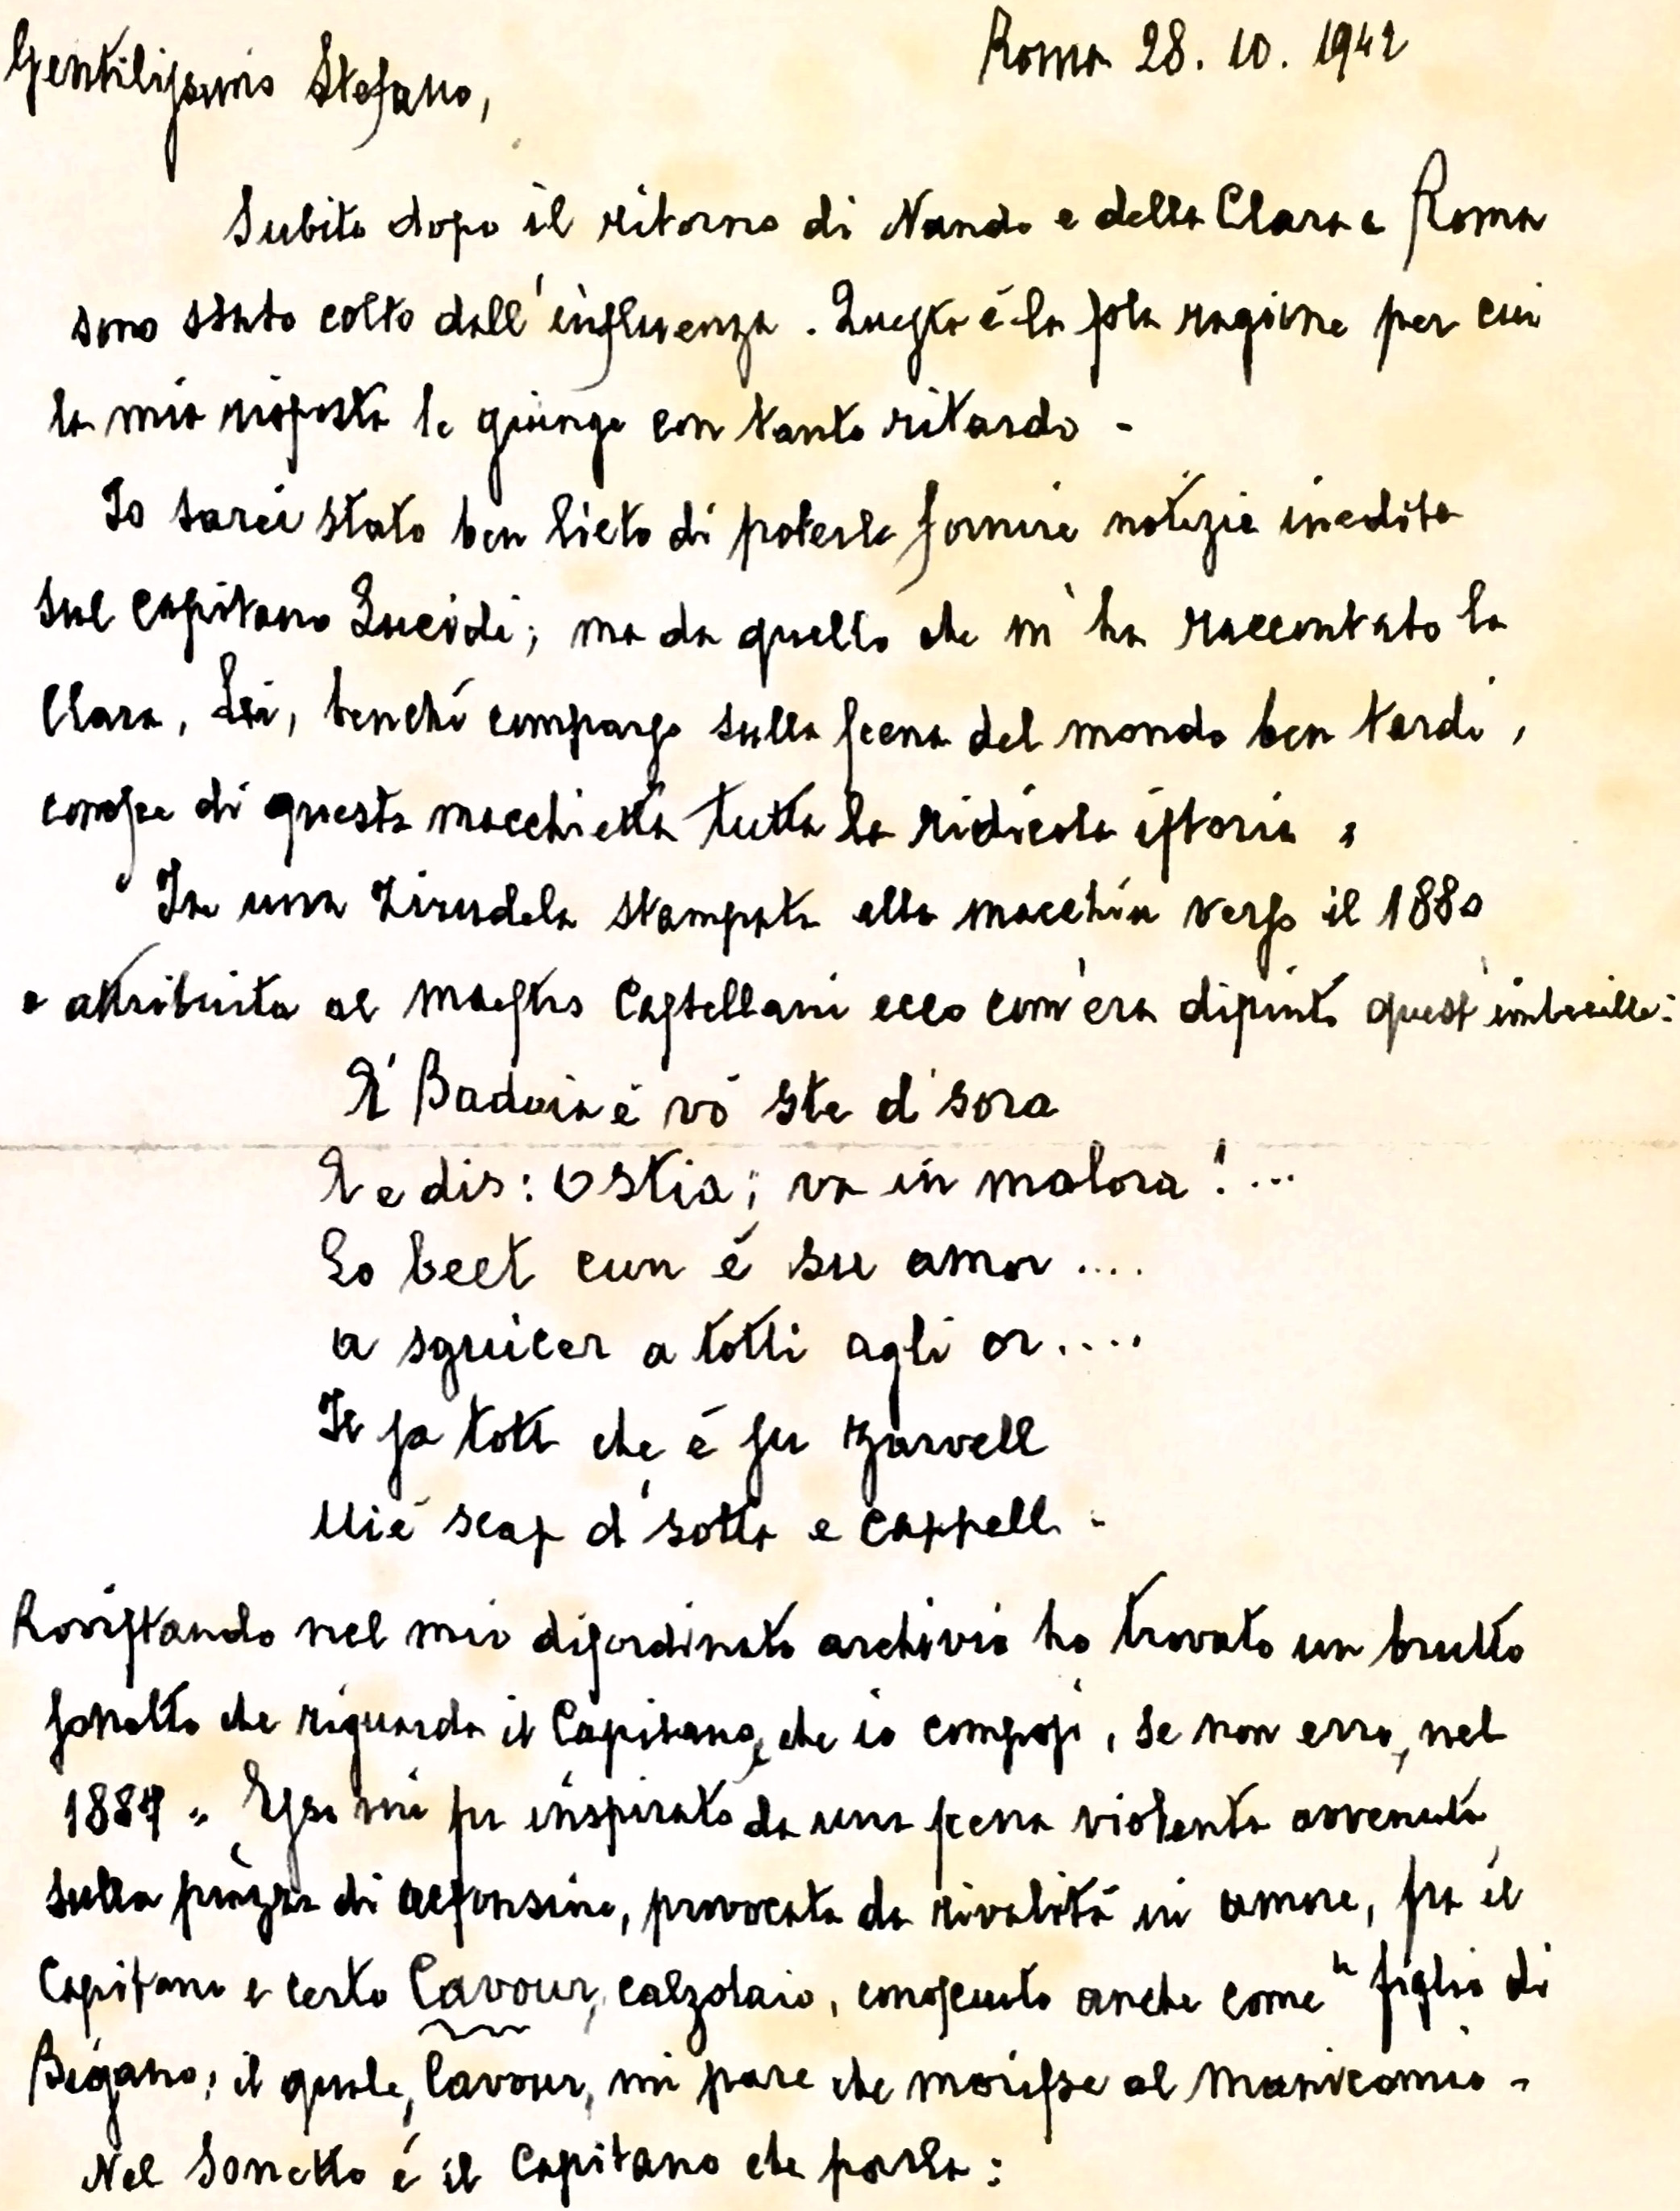
\includegraphics[width=\textwidth]{lettera}
    \caption[Lettera di Ugo De Maria]{}
    %\vspace{-0.3cm}
\end{figure}

